%intro
The ever increasing availability of cheap sensing devices and the rapidly growing number of large-scale sensor
network deployments are expanding our sensing capabilities to unprecedented levels. Many large-scale sensing projects
are being developed, from environmental monitoring to better understand changing ecosystems~\cite{neon, earthscope,
swissexp}, to weather stations trying to forecast possibly disruptive events~\cite{casa, lead}, the raizon d'\^etre of any sensing project is data. While many efforts have made to
address the networking and other infrastructure-related issues, recently there has been a lot of interest on tools to
manage, analyse and understand the sensing data, especially in real-time~\cite{stream-processing-challanges}. 

%global sensor web
Even though data coming from one sensor network deployment can be invaluable, we can expect in the future more and more
collaboration in the sensing community. Being able to access data from many different sensor networks, possibly of
different nature, is going to greatly expand the research possibilities offered by this technology. Many people believe
that is the future a \textit{world-wide sensor web} will be created~\cite{irisnet, senseweb}, in which users can query, as a single unit, vast quantities of data, from thousands of
even million of widely distributed, heterogeneous sensors. While sensor networks will be responsible of the data
collection, a cooperative pool of Internet-connected computing units will be in charge of the data processing. 
Figure~\ref{fig:wwsw} depicts this scenario.

\begin{figure}[b!]
	\centering
	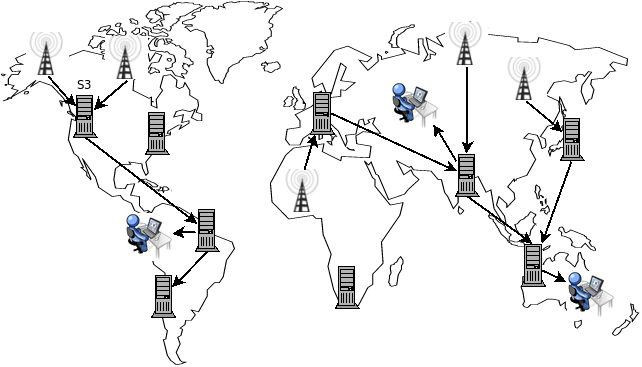
\includegraphics[width=0.75\textwidth]{img/mydissp.png}
	\caption{The \emph{World-Wide Sensor Web}, many believe, is going to be a shared infrastructure, through which it will be able to
query a large set of sensors and to process the data they produce.}
	\label{fig:wwsw}
\end{figure}

%challanges
When considering such an infrastructure, there are many issues that need to be addressed to make it usable. The amount
of generated data is going to be huge and it needs to be processed reliably. Failure is going to be the common case,
both at sensor and processing level, so particular emphasis must be given to the \emph{dependability} of the system. Also, even
though the data is highly heterogeneous, the access interface should be consistent, thus the need of as common language
to express queries. Also, not all the data is probably going to be shared among all users, there is then the need for a mechanism to
finely tune the collaboration policies. Finally, because of the enormous amount of base sources, constantly changing in
number and possibly in location, discovering the sources is also going to be problem that need to be addressed.
In the following sections I will disccus in more detail the issues that a global sensing infrastructure faces in terms
of \emph{scalability, dependability, query language, privacy and access control} and \emph{resource discovery}.

\subsection{Scalability}
%why scalability	
The concept of \emph{scalability} connotes the ability of a system to accommodate an increasing number of elements or objects, to
process growing volumes of work gracefully, and/or to be susceptible to enlargement~\cite{scalability}.
A global sensing infrastructure is going to deal with a very large number of base sources, possibly in the order of
hundreds of thousands or even millions~\cite{dependable-is-sensing, mortar-short}. Also, not only the number of sources is large, but also the number of supported queries. 
If we assume the system to be a common infrastructure for numerous sensor networks, we can expect the number of users 
to be also large. Moreover, these queries will probably be executed over long intervals of time~\cite{stream, irisnet} since 
the observed phenomena may span for weeks or even months. Given these constraints, it is evident how scalability must
lead the design of such a system. 

%distributed
A centralized approach would struggle to meet these requirements~\cite{stream}. A better approach is to employ a
distributed system~\cite{irisnet, borealis-design, mortar-long}.  This approach
is intrinsically more suitable and presents a number of advantages. First, because sensors are going to be geographically
distributed all over the world, also the processing nodes should be. Having a number of distributed computing sites allow the allocation of operators in
processing units in strategic locations, reducing the amount of data that needs to be moved within the
infrastructure~\cite{sbon, placement_strategies}.
A distributed approach also allows for incremental resource provisioning, as the system grows more computing nodes can
be added to meet the increased processing needs. This approach is also more robust, being no single point of failure.
Finally, a distributed design offers better fault-tolerance and availability, since some operators composing the query
can be run in parallel at different locations.~\cite{borealis-fault_tolerance, borealis-fast_and_ha, borealis-fast_and_reliable}.

\subsection{Dependability}
%failure unavoidable
\emph{Dependability}~\cite{dependability}, in this context, refers to the ability of the system to tolerate and resilience failure.
In such an Internet-scale infrastructure failure is the norm, rather than the exception~\cite{correlated-failures,
failure-analysis}. When issuing queries over such a large number of sensors geographically distributed worldwide, it is infeasible that all of them will be available and
able to provide data correctly. A certain number of them is going to fail or be unreachable. Failure is also going to be
common in the processing infrastructure. Being composed of a large number of computing nodes, it is probable that a
number of them will be unavailable at all times. Because of unpredictable variation in the rate or complexity of the
data streams, a node might become overloaded and thus unable to process all the incoming data~\cite{dist-net-mon}. Also, It might be
unreachable because of a network partition or even experience a software or system crash. An Internet-scale 
stream processing system should be designed to be able to operate under constant partial failure. 

%dependability - metrics
In such a system, \textit{dependability} should a key design principle. The system should support \emph{introspection}:
the ability to reason about the its performance and behaviour. It should be able to provide the user with some metrics
describing the achieved quality-of-services. Even though perfect processing would be desirable, in a real-world deployment an approximate result is
probably the best the system can provide. Nevertheless, the user should be aware of any degradation in the quality of
the processing, in order to reason on the goodness of the result data. Many application can tolerate a certain degree
of \emph{controlled degradation}~\cite{dissp-challanges} of result quality: a query averaging temperatures over a wide
area can accept the loss of some sensor data, as long as this loss is considered marginal and does not greatly affect
the final result.

%dependability - mitigation
Also, even though perfect processing might be unachievable, the system should take all the necessary measures to
reduce the occurrence of failure and to mitigate its impact on the processing~\cite{dependable-is-sensing,
borealis-fault_tolerance}. A major role in this regard is played by \emph{operator replication}. 
The system can identify the most important operators in a query and run them concurrently. In this way, if a node
hosting a part of the query fails, one of its replicas can be employed instead, without any damage to the processing.
Replication is not only useful to increase the dependability of the system, but can also improve its performance by
running the replicas in competition (i.e. to reduce latency)~\cite{borealis-fast_and_ha, borealis-fast_and_reliable}.


%Maintaining this replicas on sync might be a major challenge as tuples might be delayed or be missing due to failure. 
%The authors of~\cite{dependable-is-sensing} propose free the system from such a burden and to employ \textit{free-running} operators. 
%In this case though, the system has to be able to identify which is the replica producing the best results, this can be achieved by the mean of quality-metrics.

\subsection{Query Language}
A key goal of a global sensing infrastructure is to provide a unified interface over an heterogeneous set of sensors.
While the input data can be of many different kinds, there should be a simple and homogeneous way of accessing it.
There is then the need for a standard query-processing language, giving a standard access interface to the system, while
hiding the underlying complexity of the infrastructure. Even though the actual language may vary, it is common to query the
system using a relational approach. This is quite intuitive as it allow the user to describe the desired result in easy
terms and let the system take care of the underlying details. The de-facto standard query language for stream
processing system is the \textit{Continuous Query Language} (CQL)~\cite{cql}, which has been further standardized in~\cite{streamsql}.
A more detailed explanation of query languages can be found in Chapter~\ref{ch:language}.

\subsection{Privacy and Access Control}
%need for policies
A global sensing infrastructure has, as its inputs, many different sensor networks deployed and administered by different
organisations~\cite{irisnet, stream-processing-challanges}. In such a scenario, it is expectable that not all the data
will be accessible to all the users. Even
though the bulk of the sensing data can be publicly accessible, some will carry sensible information and its
availability might be restricted. Developing mechanisms to protect to control the access to the data, managing its
security, and regulate its use is one of the major challenges for as global sensor web~\cite{sn-security}. There should be a way for
content providers to restrict to establish policies over the accessibility of their data. 

%We can expect a number of peering agreement to be established, similarly to the ones now governing the relationships among AS on the Internet today. 

%privacy
Privacy preservation is another challenge faced by such systems. In many cases, sensible information about individuals
might be unintentionally exposed through data streams. Health care data is the prime example of sensible data, and also location is often conidered as private.
While it might be acceptable to share this kind of data, it is of vital importance that the privacy of the
individuals is preserved. Besides these obvious cases, there are a number of subtle privacy issues arising from the
sharing of sensor data. For example, an adversary gaining access to temperature readings in a house might be able to
infer details about the inhabitants's private activities~\cite{temp-privacy}. 


\subsection{Data Source Discovery}
\label{sec:source_discovery}
%why is difficult
Another important issue faced by any global sensing infrastructure is \textit{source discovery}. Considering the
diversity of sensors, both in sensing capabilities and location, it is expectable that any query will be
interested only in a subset of the grand total of input sources. A query is most probably going to process data coming
from sensors in the same region or with the same capabilities. It is then important to be able to obtain these subsets
based on their characteristic in an intuitive and scalable way. Finding the correct source base for a query is not an
easy task, if we consider the number of characteristics on which the distinction can be made, and also the number of the
sources themselves. If we also consider the sources to be mobile, like in the case of sensors embedded in smartphones
for instance, it is evident how the problem is not of easy solution. I do not intend to address this problem, instead I
will make use of one of the available solutions for the discovery of data sources in DISSP.

%howto
There is then the need for a reliable, scalable \textit{discovery service}, to obtain a list of input sources with the
desired characteristics.  In general all the research prototype bypass
this problem by assuming such a system is in place~\cite{borealis-design, stream, mortar-long}, since the solution of the discovery problem is very challenging on
its own. There are, though, a number of solutions possible, some directly targeted to sensor networks and other more
generically focused on resource discovery. One of the most intuitive sensor discovery interface is SenseMap~\cite{sensemap}. 
It is a map where sensors are displayed in their geographical location, exposing also their sensing capabilities. The
user can easily select all the sensors in an area with certain characteristics, or can click on the single sensors.
This is probably the best example of selection tool specifically designed for sensors. 

%other fields
Even though SenseMap is a good solution for the source discovery and selection problem, it might not be appropriate in
all cases. For instance, if the number of sources is very large and their location is not known a priori, other more
descriptive mechanisms might be more suitable. In this case a declarative approach would be more suitable, letting the
user describe the characteristics of the input sources. The solution here is not quite obvious, but there are a number of
approaches that can be borrowed from other projects. Sword~\cite{sword} is the PlanetLab resource discovery system. It is
based on a \emph{distributed hash table} (DHT) and focuses on the finding a suitable subset of machines for an experiment, given a number of attribute constraint, both
per-node and inter-node. \\
Another discovery approach could be borrowed from PIER~\cite{pier1, pier2}. Using this system, sources can be places in the internal DHT based on their attributes.
By issuing a select query specifying a set of attributes it would be possible to scalably retrieve the desired input
sources. In the field of Grid computing, we find also solutions for resource selection. A particularly scalable
solution is proposed in~\cite{rss-costa}, with their Autonomous Resource Selection Service. This is again a DHT based
approach, able also to address range queries, where the internal routing tables are updated using epidemic protocols. 


